\section{Sign Test}
Sign test is like the nonparametric version of the paired or one sample t-test. The primary interest is centered on the location (median) of a
population.

There are two scenarios, or say, two kinds of dataset, to apply Sign Test.
\begin{itemize}
	\item \textbf{Paired Data}: pairs of ``pretreatment'' and ``posttreatment'
observations. We would like to inference the existence of a shift in location due to the ``treatment''.
	\item \textbf{One-sample Data}: Observations from a single population about
whose location we wish to make inferences.
\end{itemize}

\subsection{Paired Data}

Paired Data is also known as Dichotomous Data.It consists
of n independent subjects and each subject has 2 observations. The follow is an example of the paired data.

\begin{figure}[H]
	\centering
	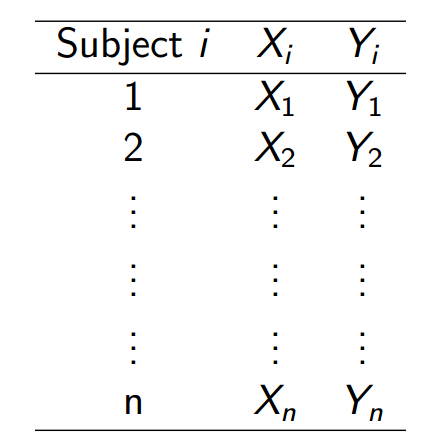
\includegraphics[width=0.2\linewidth]{fig/paired-data}
	\caption{}
	\label{fig:paired-data}
\end{figure}

\subsection{Assumptions}
Let $Z_i = Y_i - X_i$, $i = 1, \dots, n$. The difference $Z_1, \dots, Z_n$ are mutually independent, while $X_i$ and $Y_i$ can be dependent.

Each $Z_i$ comes from a continuous population (not necessarily the same one) has a common median $\theta$. The parameter $\theta$ is referred to as \textbf{the treatment effect}.
\begin{itemize}
	\item $\P(Z_i \le \theta) = \P(Z_i > \theta) = \half$
	\item $\P(Z_i - \theta \le \theta) = \P(Z_i - \theta > 0) = \half$
\end{itemize}

\subsection{Hypothesis Test}
\[H_0: \theta = 0\]
The null hypothesis is that each of the distributions (not necessarily the same) for the
differences (post-treatment minus pre-treatment observations) has
median 0, corresponding to no shift in location due to the
treatment.

The \textbf{sign statistic} is the number of positive $Z_i$'s, $i = 1, \dots, n$.
\[T = \sum_{i=1}^{n} I_{Z_i > 0}\]
,where
\[I_{Z_i > 0} = 
\begin{cases}
	1, ~\text{if $Z_i > 0$}\\
	0, ~\text{if $Z_i \le 0$}
\end{cases}\]

Under $H_0$, we have $\P(I_{Z_i > 0} = 1) = \P(Z_i > 0) = \half$. Then random variable $I_{Z_i > 0}$ follows a Bernoulli distribution with $p= \half$. So the sign statistic $T$ follows a binomial$(n, \half)$ distribution. So $\E T = \frac{n}{2}$, $\Var T = \frac{n}{4}$.

Usually there are two kinds of test to apply:
\begin{itemize}
	\item Exact Test: calculate $p$-value based on binomial distribution.
	\item Asymptotic Test: calculate $p$-value based on the central limit theorem, where the standaried sign statistic is sampled from the the stander normal distribution when the sample size is large enough ($n > 30$). $\frac{T - \frac{n}{2}}{\sqrt{\frac{n}{4}}} \> N(0, 1)$ as $n \> \infty$.
\end{itemize}

\subsection{Right-tailed Test}
\subsection{Left-tailed Test}
\subsection{Two-tailed Test}